%--------------------------------------------------------------------
%
%Mustervorlage fuer eine Aufgabe
%
%--------------------------------------------------------------------
%
%Ueberschreiben der automatisch erzeugten Aufgabennummer
%Die folgende Aufgabennummer ergibt sich aus dem Stand des
%Z�hlers + 1
%\setcounter{chapter}{0}
%
\chapter{}\label{ex:aufg2}
%
%Teilaufgabe 1
%
\section{}\label{sec:aufg2a}
%

%
%--------------------------------------------------------------------
%
%Teilaufgabe 2
%
\section{}\label{sec:aufg2b}
%

%
\section{}\label{sec:aufg2c}
%

%
\section{}\label{sec:aufg2d}
%
Wir nutzen die Formel 5.9 aus dem Vorlesungsskript.
\begin{equation}
U_a = R_a I_a + L_a \frac{dI_a}{dt} + U_I
\label{for:formel1}
\end{equation}
Da \[U_I = 0\]kommen wir zu folgender Formel:
\begin{equation}
I_a = \frac{U_a - L_a \frac{dI_a}{dt}}{R_a}
\label{for:formel2}
\end{equation}
%
\newline
\newline
%
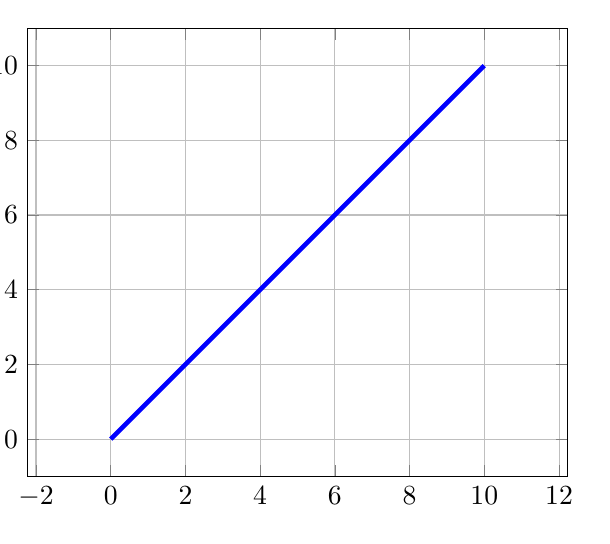
\begin{tikzpicture} [trim axis left]
\begin{axis}[domain=0:10,
samples=100,
enlarge x limits=false,
grid=both,
no markers,
axis equal]
\addplot[blue, ultra thick] (x,{\x});
\end{axis}
\end{tikzpicture}



%\begin{tikzpicture}

\begin{axis}[xmax = 10, ymax = 15, samples=100]
\addplot[blue, ultra thick] (x,x*x)
\end{axis}

\end{tikzpicture}

%Alle bisherigen Bilder einf�gen und einen Seitenumbruch erzwingen
\clearpage
